%%%%%%%%%%%%%%%%%%%%%%%%%%%%%%%%%%%%%%%%%%%%%%%%%%%%%%%%%%%%
%%% ELIFE ARTICLE TEMPLATE
%%%%%%%%%%%%%%%%%%%%%%%%%%%%%%%%%%%%%%%%%%%%%%%%%%%%%%%%%%%%
%%% PREAMBLE 
\documentclass[9pt,lineno]{elife}

\usepackage[export]{adjustbox}
\usepackage{lscape}
\usepackage{afterpage}
\usepackage{hyperref}
\hypersetup{
    colorlinks=true,
    linkcolor=blue,
    filecolor=magenta,      
    urlcolor=cyan,
}

\newcommand{\sgcomment}[1]{\textcolor{blue}{SG: #1}}
\newcommand{\luke}[1]{\textcolor{blue}{Luke: #1}}
\newcommand{\todo}[1]{\textcolor{blue}{*#1*}}
\newcommand{\alex}[1]{\textcolor{red}{Alex: #1}}
%%%%%%%%%%%%%%%%%%%%%%%%%%%%%%%%%%%%%%%%%%%%%%%%%%%%%%%%%%%%
%%% ARTICLE SETUP
%%%%%%%%%%%%%%%%%%%%%%%%%%%%%%%%%%%%%%%%%%%%%%%%%%%%%%%%%%%%
\title{Legacy Data Confounds Modern Genomics Studies}

\author[1,2]{Luke Anderson-Trocm\'e}
\author[1,2]{Mathieu Bourgey}
\author[3]{Fumihiko Matsuda}
\author[1,2]{Simon Gravel}

\affil[1]{Department of Human Genetics, McGill University, Montreal, QC H3A 0G1, Canada}
\affil[2]{McGill University and Genome Quebec Innovation Centre, Montreal, QC H3A 0G1, Canada}
\affil[3]{Center for Genomic Medicine, Graduate School of Medicine, Kyoto University, Kyoto 606-8501, Japan}
\corr{simon.gravel@mcgill.ca}{SG}

%%%%%%%%%%%%%%%%%%%%%%%%%%%%%%%%%%%%%%%%%%%%%%%%%%%%%%%%%%%%
%%% ARTICLE START
%%%%%%%%%%%%%%%%%%%%%%%%%%%%%%%%%%%%%%%%%%%%%%%%%%%%%%%%%%%%
\begin{document}

\maketitle
\begin{abstract}
In investigating a population genetics signal, we noticed some discrepancies between the Japanese samples from the 1000 Genomes Project (1kGP) and a more recent high quality dataset.
We found that the variants causing the signal were only present in individuals with low average sequencing quality.
We identified $625\ \  p < 10^{-8}$ and $1048\ \ p < 10^{-6}$ single nucleotide polymorphisms (SNPs) that were associated to quality in the 1kGP dataset Japanese individuals.
These variants are present in nearly all of the populations from the 1kGP. 
We then turned our attention to the rest of the 1000 Genomes populations and saw that there were similar batch effects in many of these populations.
Some of these variants are being imputed onto genotype data and reach genome wide significance in recent publications.
\todo{update values for all populations}
\end{abstract}

			\section{Introduction}
		
	\subsection{Reference Cohorts}			



%The last 5 years have seen an increase in the number of individuals genotyped through private companies or medical research cohorts. 
%Larger sample sizes allow researchers to identify finer resolution statistically significant differences between groups of individuals. 
%Mutations associated to a disease can be identified by comparing the genomes of healthy individuals to those afflicted by a disease. 
%The mutations commonly found in patients and rarely in controls might be associated to the disease in question.
%However, demonstrating that these mutations are biologically relevant can be difficult.
%Especially with the increasing size of cohorts, spurious associations are increasingly becoming an issue. 
%For this reason, careful consideration must be taken when including individuals from different ancestral origins in these association studies.
%Benign mutations at high frequencies in one populations might be exceedingly rare in another population.
%Therefore, population wide differences in mutations must be included as covariates to avoid spurious associations.

%\sgcomment{This intro paragraph is much too vague -- it reads like general thoughts about genetics at large. We need to be much more concise. I would start with something like:}

The last 5 years have seen a drastic increase in the amount and quality of human genome sequence data. 
Hapmap [\cite{}], the 1000 Genomes Project [\cite{}], and the Simons Diversity project [\cite{}], for example, have made thousands of genomes publicly available for population and medical genetic analyses. 
Many more genomes are available indirectly through servers providing imputation services \cite{haplotype reference consortium} or variant frequency estimation \cite{GnomAD}. 

Many of these large datasets have been assembled over several years. 
The first sequenced genomes in the 1000 Genomes project (1kGP), for example, were sequenced \todo{10} years ago, before most of the current best technologies and analysis practices were in place. 
Because of the extraordinary value of freely available data, this early data from the 1kGP is still widely used as a reference panel for imputation, allele frequency estimations and a wide range of applications. 

Yet this data is far from perfect \sgcomment{cite papers that have pointed out issues}. 
This raises the question of whether and how such legacy data should be included in contemporary analyses alongside more recent cohorts. 
Here we point out how large and previously unreported batch effects in the early phases of the 1000 Genomes Project still lead to incorrect genetic conclusions through population genetic analyses and indirect use through prominent imputation servers.  


\subsection{Motivations}

%A genome wide mutational signature can be measured by taking the sum of all the different types of mutations in an individual. 
%\sgcomment{This is a procedural definition. You need a conceptual definition! Something like:} 

Mutations in the genome can be caused by exposure to a mutagen, defective DNA repair or errors in DNA replication.


Mutation rates depend on environmental exposure as well as variation in genetic factors like DNA proofreading and repair [\cite{}].
Some mutagens are more likely to affect a specific genomic context which therefore leaves a mutational signature [\cite{}].
It has been shown that certain types of cancer have particular mutational profiles that can be used as a diagnostic tool [\cite{}]. 

This means that the neighbouring nucleotides of a mutation can be used to gain insight into the cause of a mutation [\cite{}].
Thymine dimers caused by UV radiation were detected early on because they were highly specific and easy to study [\cite{}].
However,  signatures caused by natural variations in the sequence of proteins involved in proofreading and repair are more difficult to study because they tend to occur less frequently and are more subtle [\cite{}].
A large sample size can be used to increase statistical power to resolve some of these fine scale mutational signatures [\cite{}].
%Finer scale patterns have been reported in \todo{MORE HERE} \cite{}. 

In 2015, Harris et al reported a \todo{15\%} overrepresentation of the TCC to TTC mutation in European populations. This strong population enrichment of a mutational signature suggests important genetic or environmental differences in the history of each population, and was replicated in a different cohort \cite{}.  
Harris and Pritchard further identified distinct mutational spectra across a range of populations [\cite{}]. In particular, they identified an axis of variation within 1000 Genomes Japanese individuals. 
Such an axis of variation is intriguing because differences in mutational signatures accumulate over many generations. A systematic difference among the Japanese population would suggest sustained environmental or genetic differences across sub-populations within Japan with little to no gene flow. We therefore decided to follow up on this observation, by using a newly sequenced dataset \sgcomment{description of cohort. }

While we were unable to reproduce the heterogeneity among the Japanese population, we could trace back the source of the discrepancy between the two datasets and identified a strong and previously unreported batch effect in the 1000 Genomes Project data. We also found that this batch effect led to spurious results in a number of recently published studies. 

\sgcomment{In section ..., we...}
Here we discuss the source of the batch effect and the ways in which it contaminated a number of recent studies. Fortunately, the main conclusions of most of these studies remain supported by other data.  Yet this begs the question: When should we retire legacy data?


%\subsection{Imputation}
%Genome wide associations using large cohorts have lead to developments in the identification of rare genetic diseases as well as the risk prediction to certain types of cancer and diseases. Despite drastic reductions in cost of whole genome sequencing, it remains an expensive test for large sample sizes.
%For this reason, genotype data is often imputed to increase power for association studies in a cost effective way.

%\sgcomment{Too wordy (also, readers of Nature genetics know about imputation!: Despite drastic reduction in sequencing costs, genotyping and imputation remain a more affordable and popular approach for large-scale cohorts.}





%\sgcomment{As a style issue: you tend to write sentences without indicating the logical flow between them. It makes it hard to follow. }

	

			\section{Results}
	\subsection{A peculiar mutational signature in Japan}			
If two groups of individuals are sampled from the same population, we expect there to be little deviation in allele frequencies between the two groups. 
%\sgcomment {Here again, you are a bit procedural. It's useful to explain to the reader the logical flow of how you got to doing what you are doing:} 
Harris et al reported an excess of *AC${\rightarrow}$*CC mutations in some Japanese individuals. 
While trying to follow up on this observations in a larger cohort of 886 Japanese individuals, \todo{some info about cohort}, we did not find this particular signature.
However, when comparing the allele frequencies between the Japanese individuals from the 1kGP and this larger dataset, we observed an unusually large number of private single nucleotide polymorphisms (SNPs), only found in one of the two groups. 
These mismatches were maintained after filtering for low-quality regions of the human genome and standard metrics such as Hardy-Weinberg equilibrium

Once mismatch sites were removed from the 1kGP data, the  *AC${\rightarrow}$*CC signal disappears \ref{SFS}, suggesting a technical artifact rather than a population structure effect. Regressions against different quality metrics provided by the 1kGP revealed that mean mapping quality per mapped base pair was an excellent correlate with prevalence of the  *AC${\rightarrow}$*CC mutational signature in 1kGP, with low-quality individuals showing elevated rates of the signature. (\sgcomment{show supplementary Figure where you did the correlations})
 
 Thus sequences with low mappability harbour mutations that reproduce poorly across studies and exhibit a particular mutational signature. 

\begin{figure}
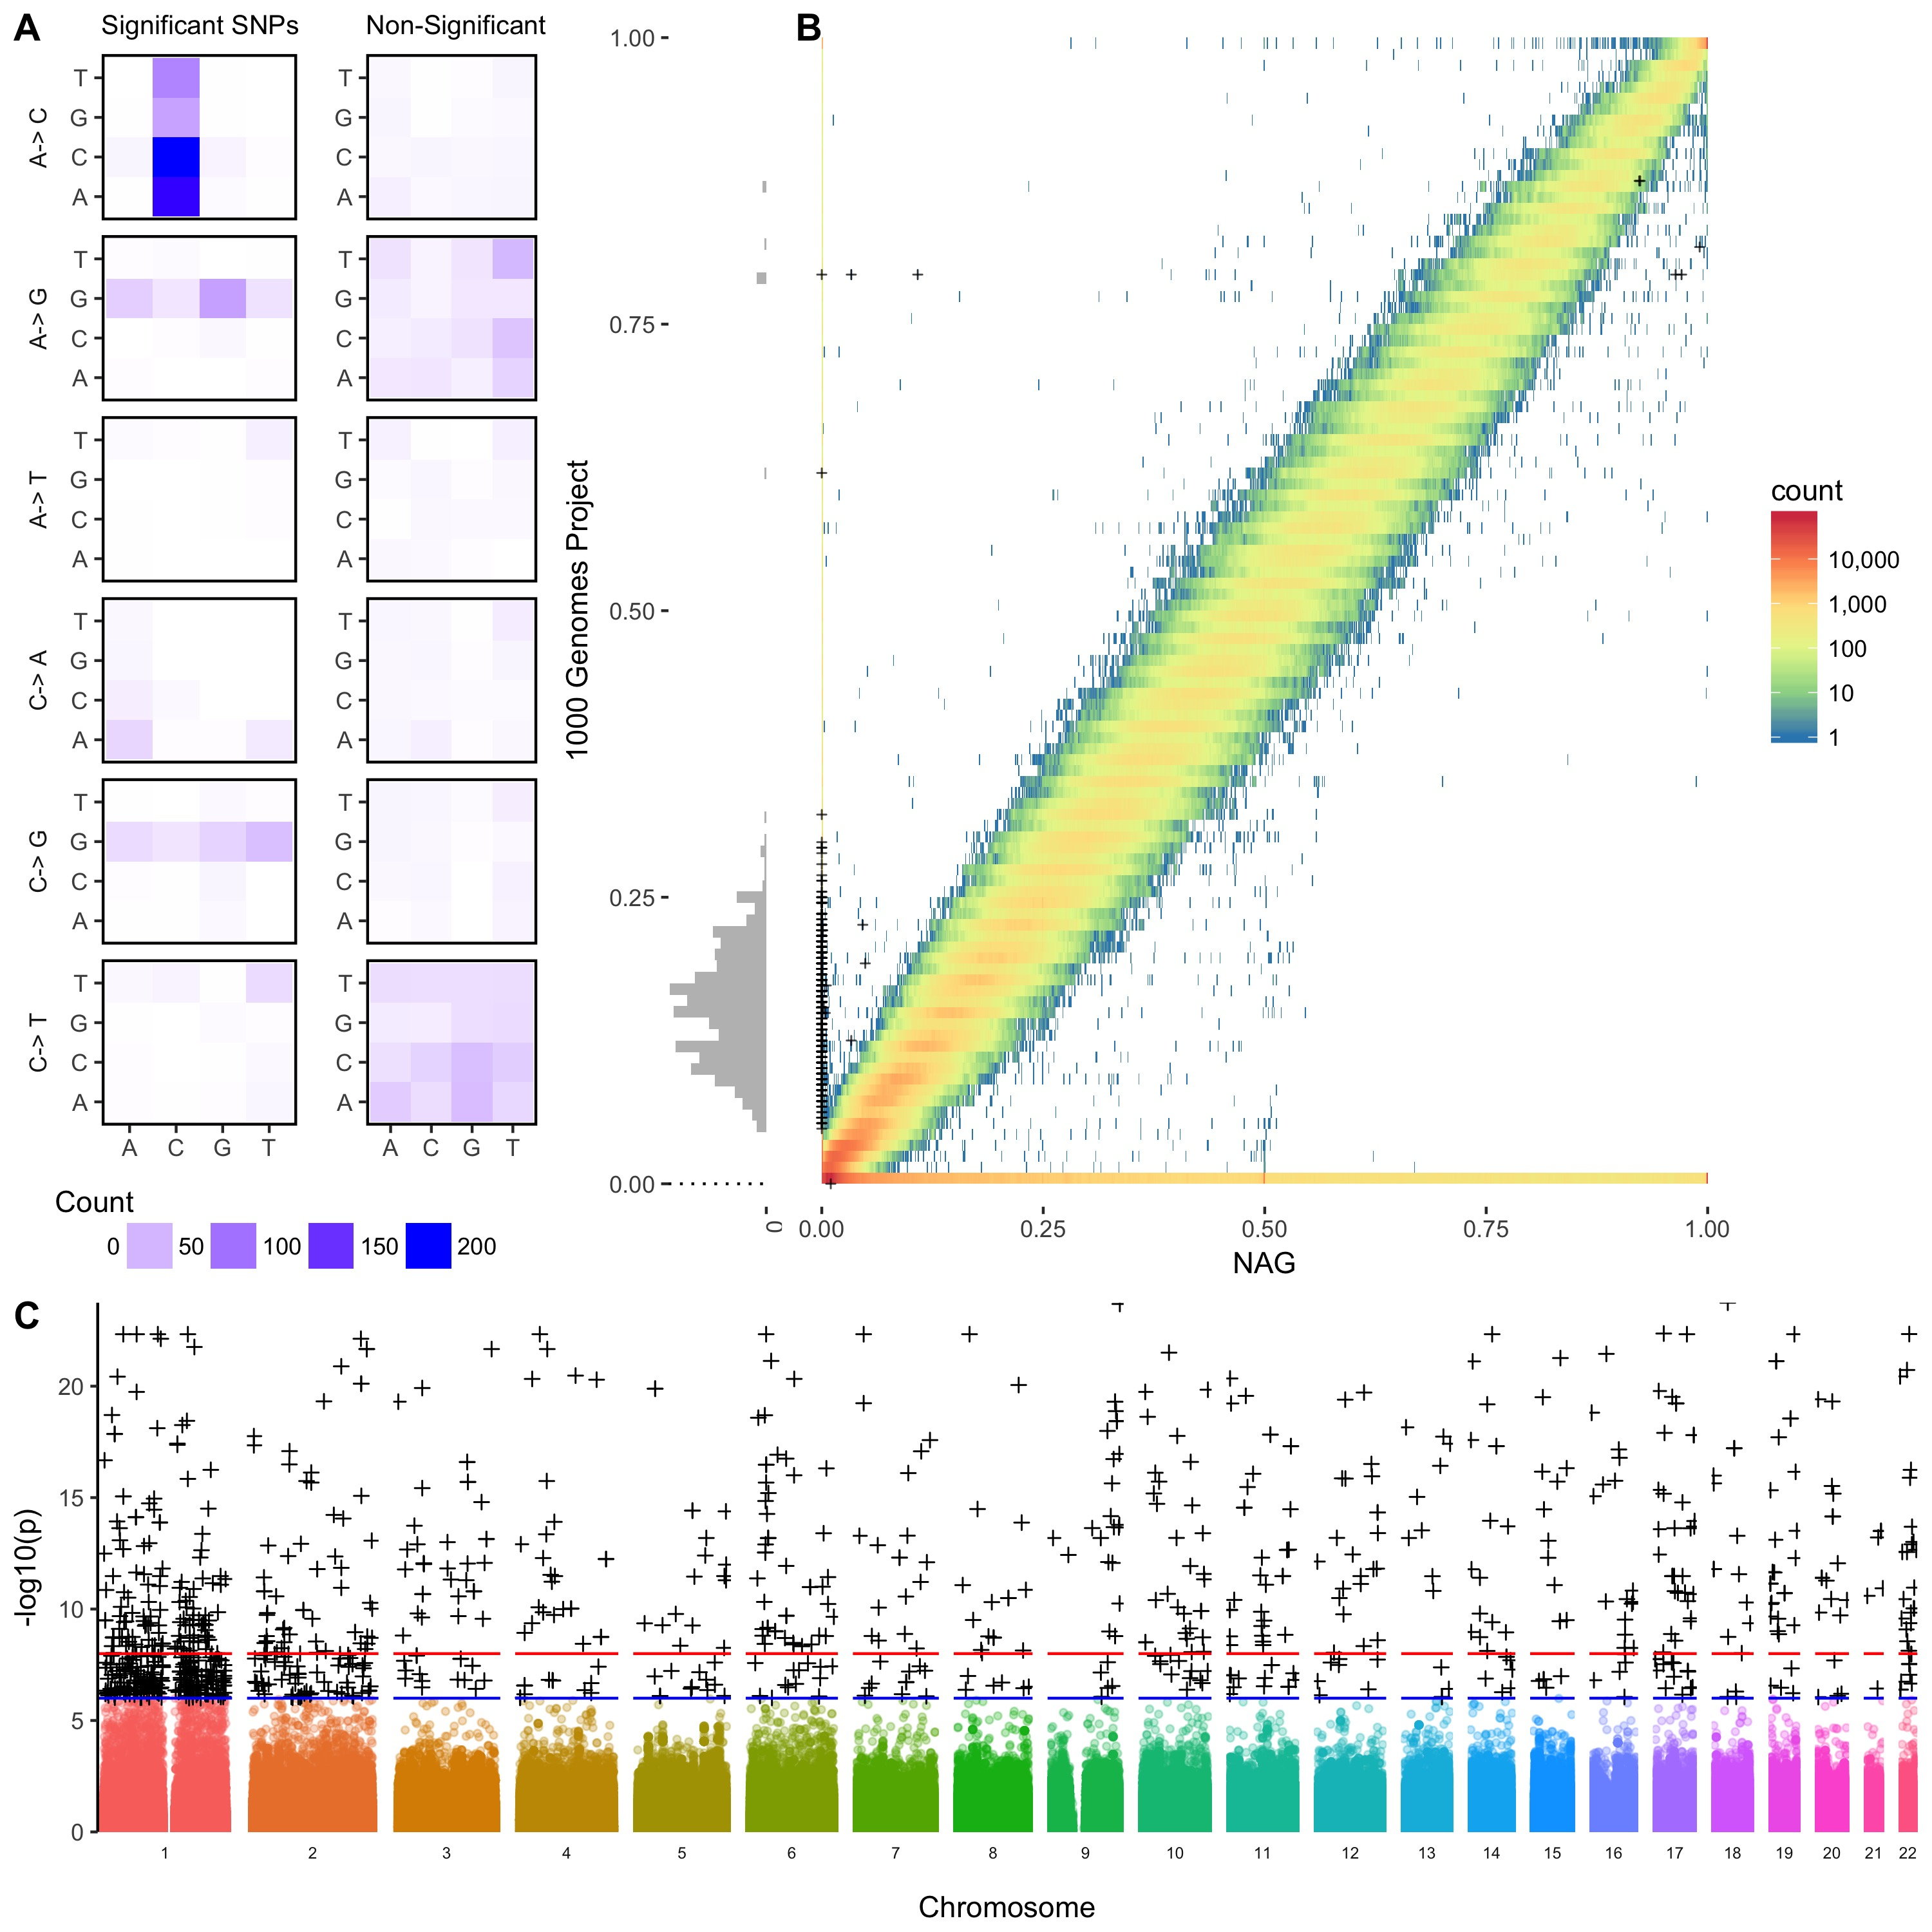
\includegraphics[width=\hsize,keepaspectratio]{Figure1.jpg}
\caption{
\textbf{A} 
Joint frequency spectrum plot of the Japanese from the 1000 Genomes Project and a more recent dataset.
Crosses ( + ) are variants that reached genome wide significance in a GWA of sequencing quality. 
The histogram on the left of the plot is the distribution of significant variants. 
The lowest frequency variant able to reach genome wide significance is 5\%.
\textbf{B} 
Mutation spectrum of the 1048 variants that reached a genome wide significance with a p value less than in a GWA of sequencing quality. 
There is a \todo{significant} enrichment in *AC${\rightarrow}$*CC mutations. 
\textbf{C} 
Genome wide association of the average quality of mapped bases for the 104 Japanese individuals included in the 1000 Genomes Project. This GWA study identified $625\ \  p < 10^{-8}$ and $1048\ \ p < 10^{-6}$ SNPs that were associated to the average quality of SNPs mapped for an individual
The same analysis was performed independently for each of the populations in the 1000 Genomes Project. }
 \label{SFS}
\end{figure}

To identify SNPs that are associated with low quality, we performed a genome-wide association (GWA) study  \ref{SFS}. 
GWA studies are commonly used to find genomic regions associated to biologically relevant traits. In this case, we are using this analysis in a more unconventional way to identify regions of the genome that are associated to biologically irrelevant traits like SNPs associated to individuals with low quality.
 
Using the linear GWA study function offered by PLINK, we were able to identify $625\ \  p < 10^{-8}$ and $1048\ \ p < 10^{-6}$ SNPs that were associated to the average quality of SNPs mapped for an individual \ref{SFS}.  This GWA study included 104 individuals, \todo{000} of them were sequenced in phase 1 while the rest were sequenced in phase 3 of the 1000 Genomes Project.
The variants that are associated to the quality of mapped bases have an enrichment in *AC${\rightarrow}$*CC mutations. 

\alex{Having trouble following the first three sentences}
Despite removing the variants identified as being low quality, the signal persists. 
When we remove the variants significantly associated to low quality, the enrichment in *AC${\rightarrow}$*CC mutations remains present, but \todo{less} significant. 
When we remove individuals with average quality of mapped SNPs below 30, the signal goes away. 
We suspect that this has to do with the lack of power we have for more rare alleles. 
The lowest frequency variants that are significantly associated to quality are at 5\%. 
When we remove all the variants above 1\% in 1kGP but missing from the NAG data, the signal disappears.
This suggests that while the GWA approach can identify some of the low hanging bad apples, there are likely more of these false positives nested inside these legacy cohorts. 

One way to assess the validity of these unusual variants is to see if they are present in a higher quality dataset. Upon comparing the Japanese 1000 Genomes cohort to a higher quality and larger cohort, we identified \todo{000} more variants that are beyond the expected frequency spectrum deviation for individuals from the same population. 

	\subsection{Sequencing quality over time}
We turned our attention to the other populations in the 1kGP, we found that the sequencing done in phase 1 was more variable and overall tended to include lower quality sequencing data \ref{MapQual}.
The sequencing quality of individuals increases over time \ref{MapQual}. 
By 2011 the sequencing quality seems to level off, this also coincides with the phasing out of older sequencing technologies. 
\begin{figure}
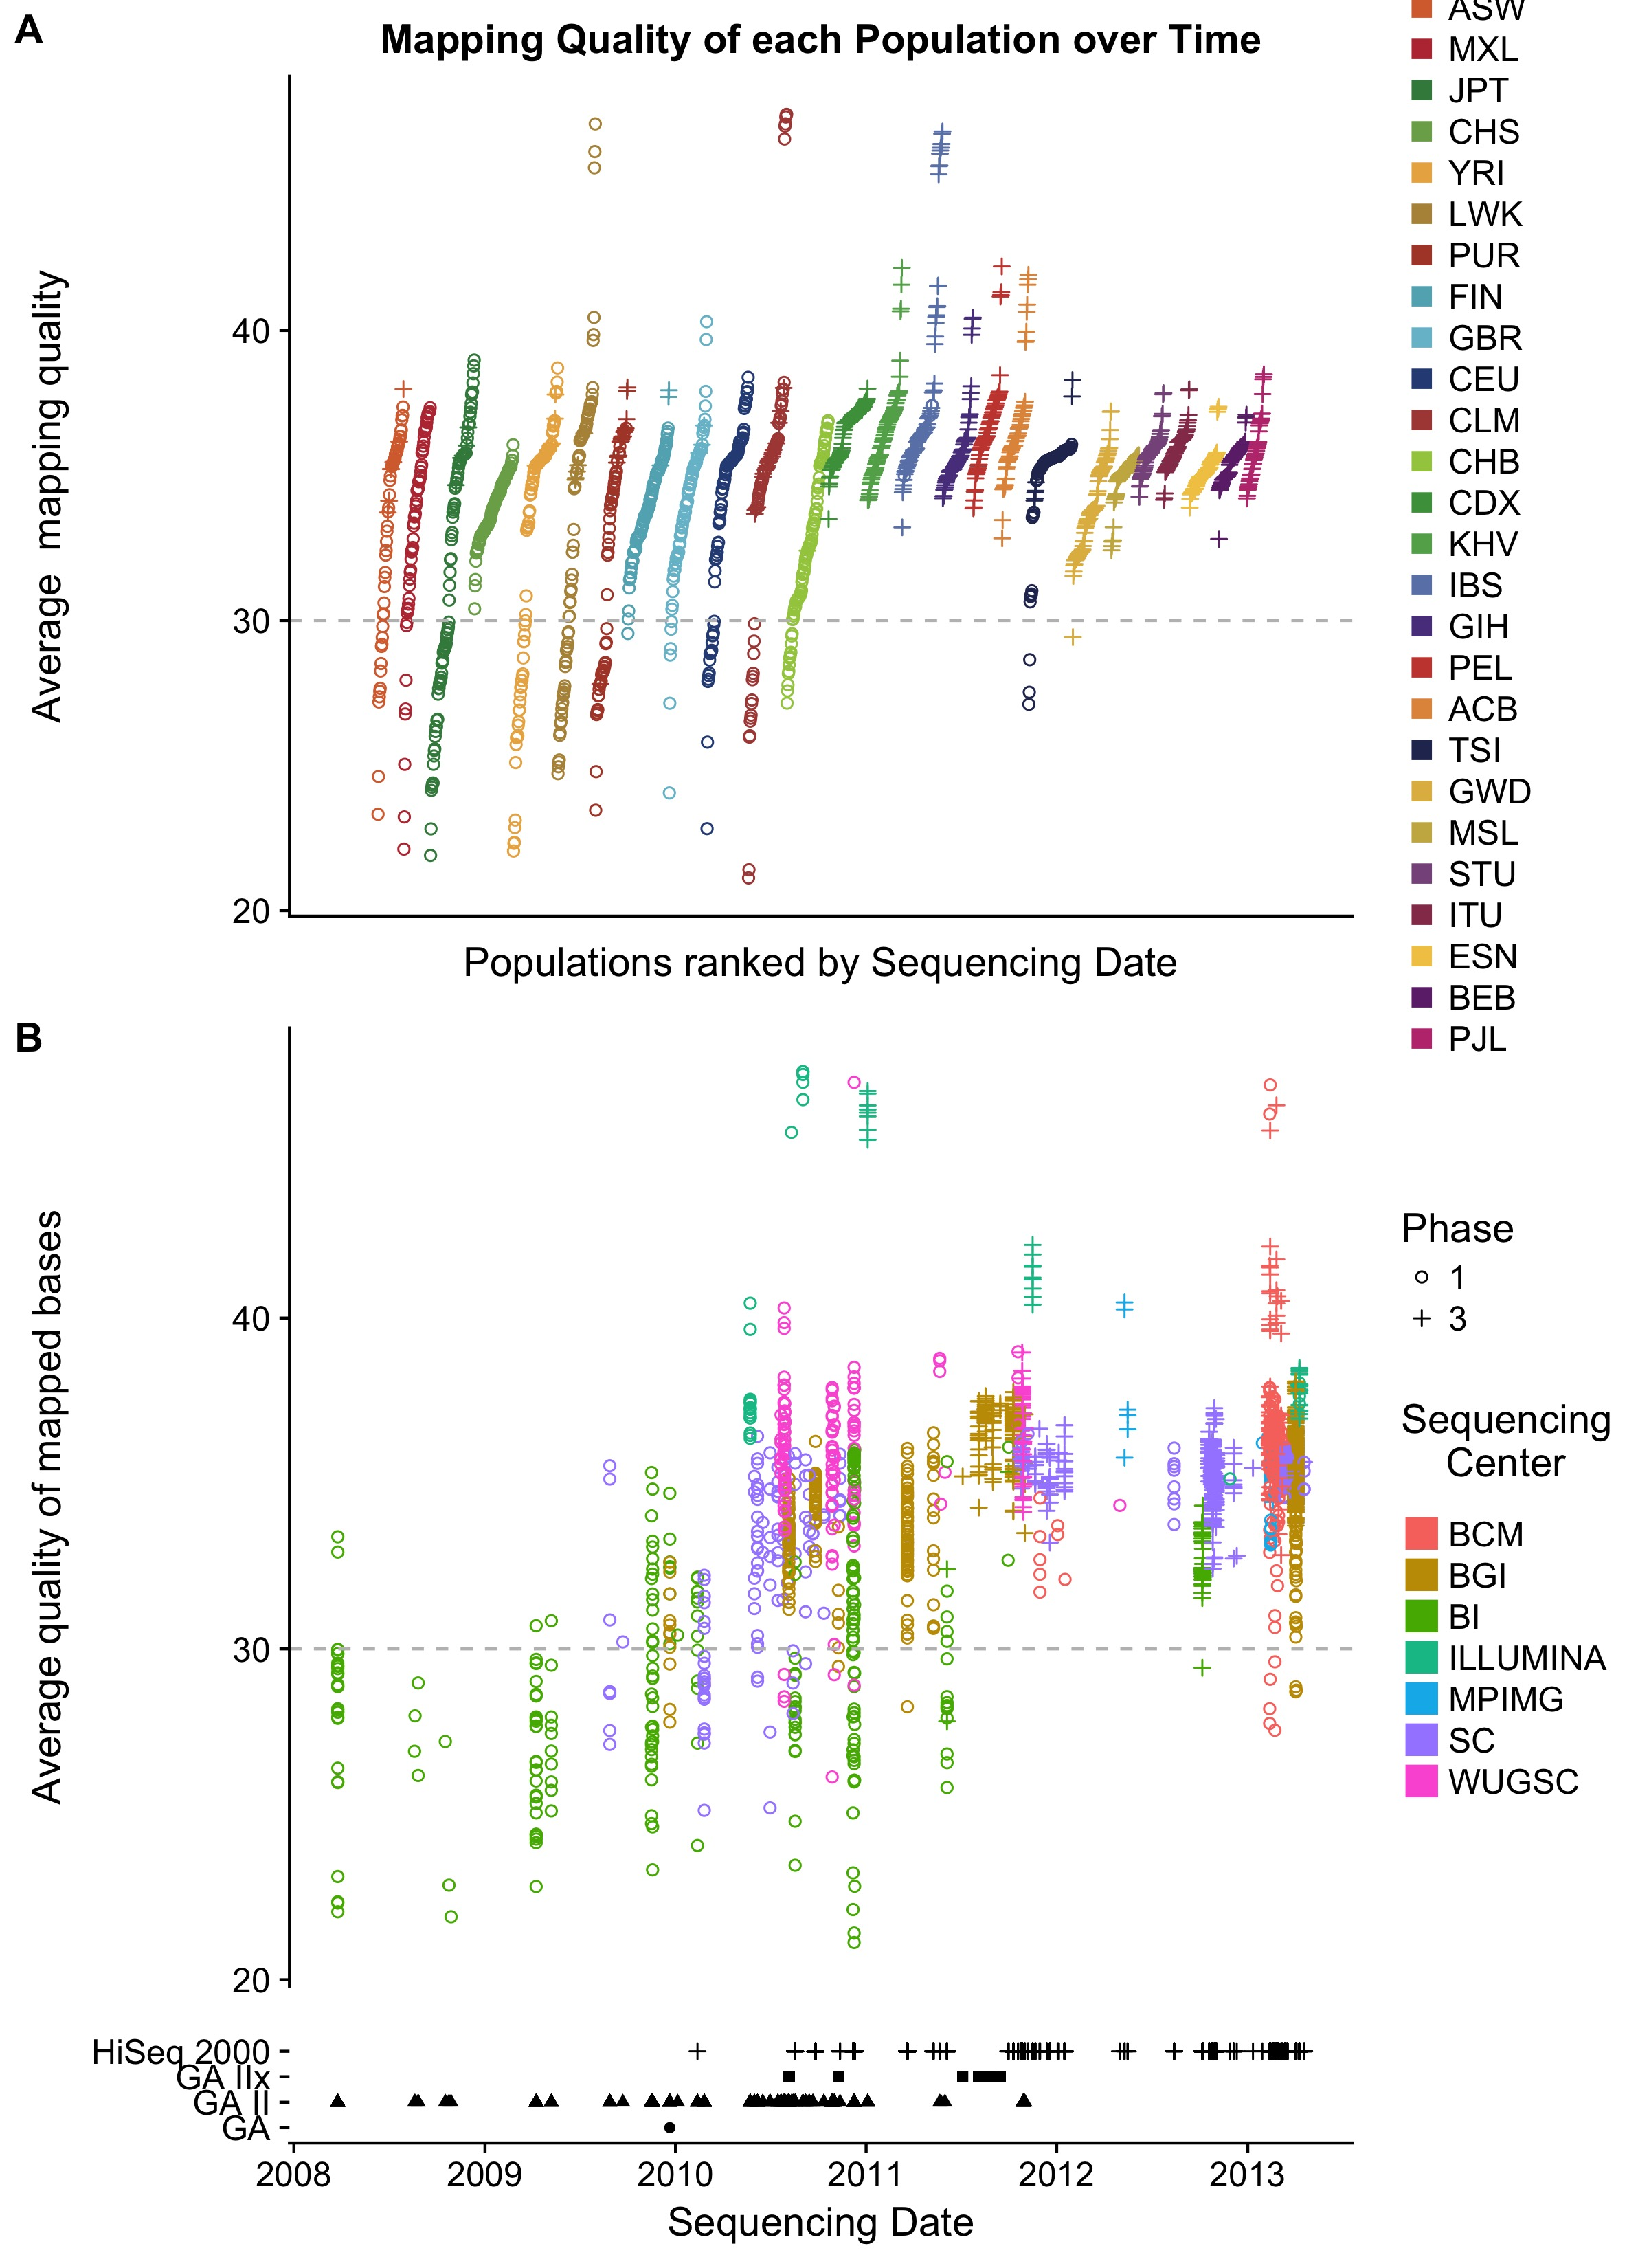
\includegraphics[width=\hsize,keepaspectratio]{MapQualOverTime.jpg}

\caption{\textbf{A} The average mapping quality of each individual per population included in the 1000 Genomes sequencing project. The x-axis is ranked by populations with the lease to the most variance, followed by average mapping quality per individual. \textbf{B} Same data as in \textbf{A} except the x-axis is sorted by sequencing date. The colors indicate the sequencing centers that produced the data for each individual.}
\label{MapQual}
\end{figure}


	\subsection{Overlap of significant SNPs}
Comparing the results of each independent GWA study, we were able to identify over \todo{0000} variants that were independently associated to low quality in multiple populations. This confirmation using more than one GWAS is a strongly suggests that these variants might not be genuine \ref{Figure3}. 

\begin{figure*}
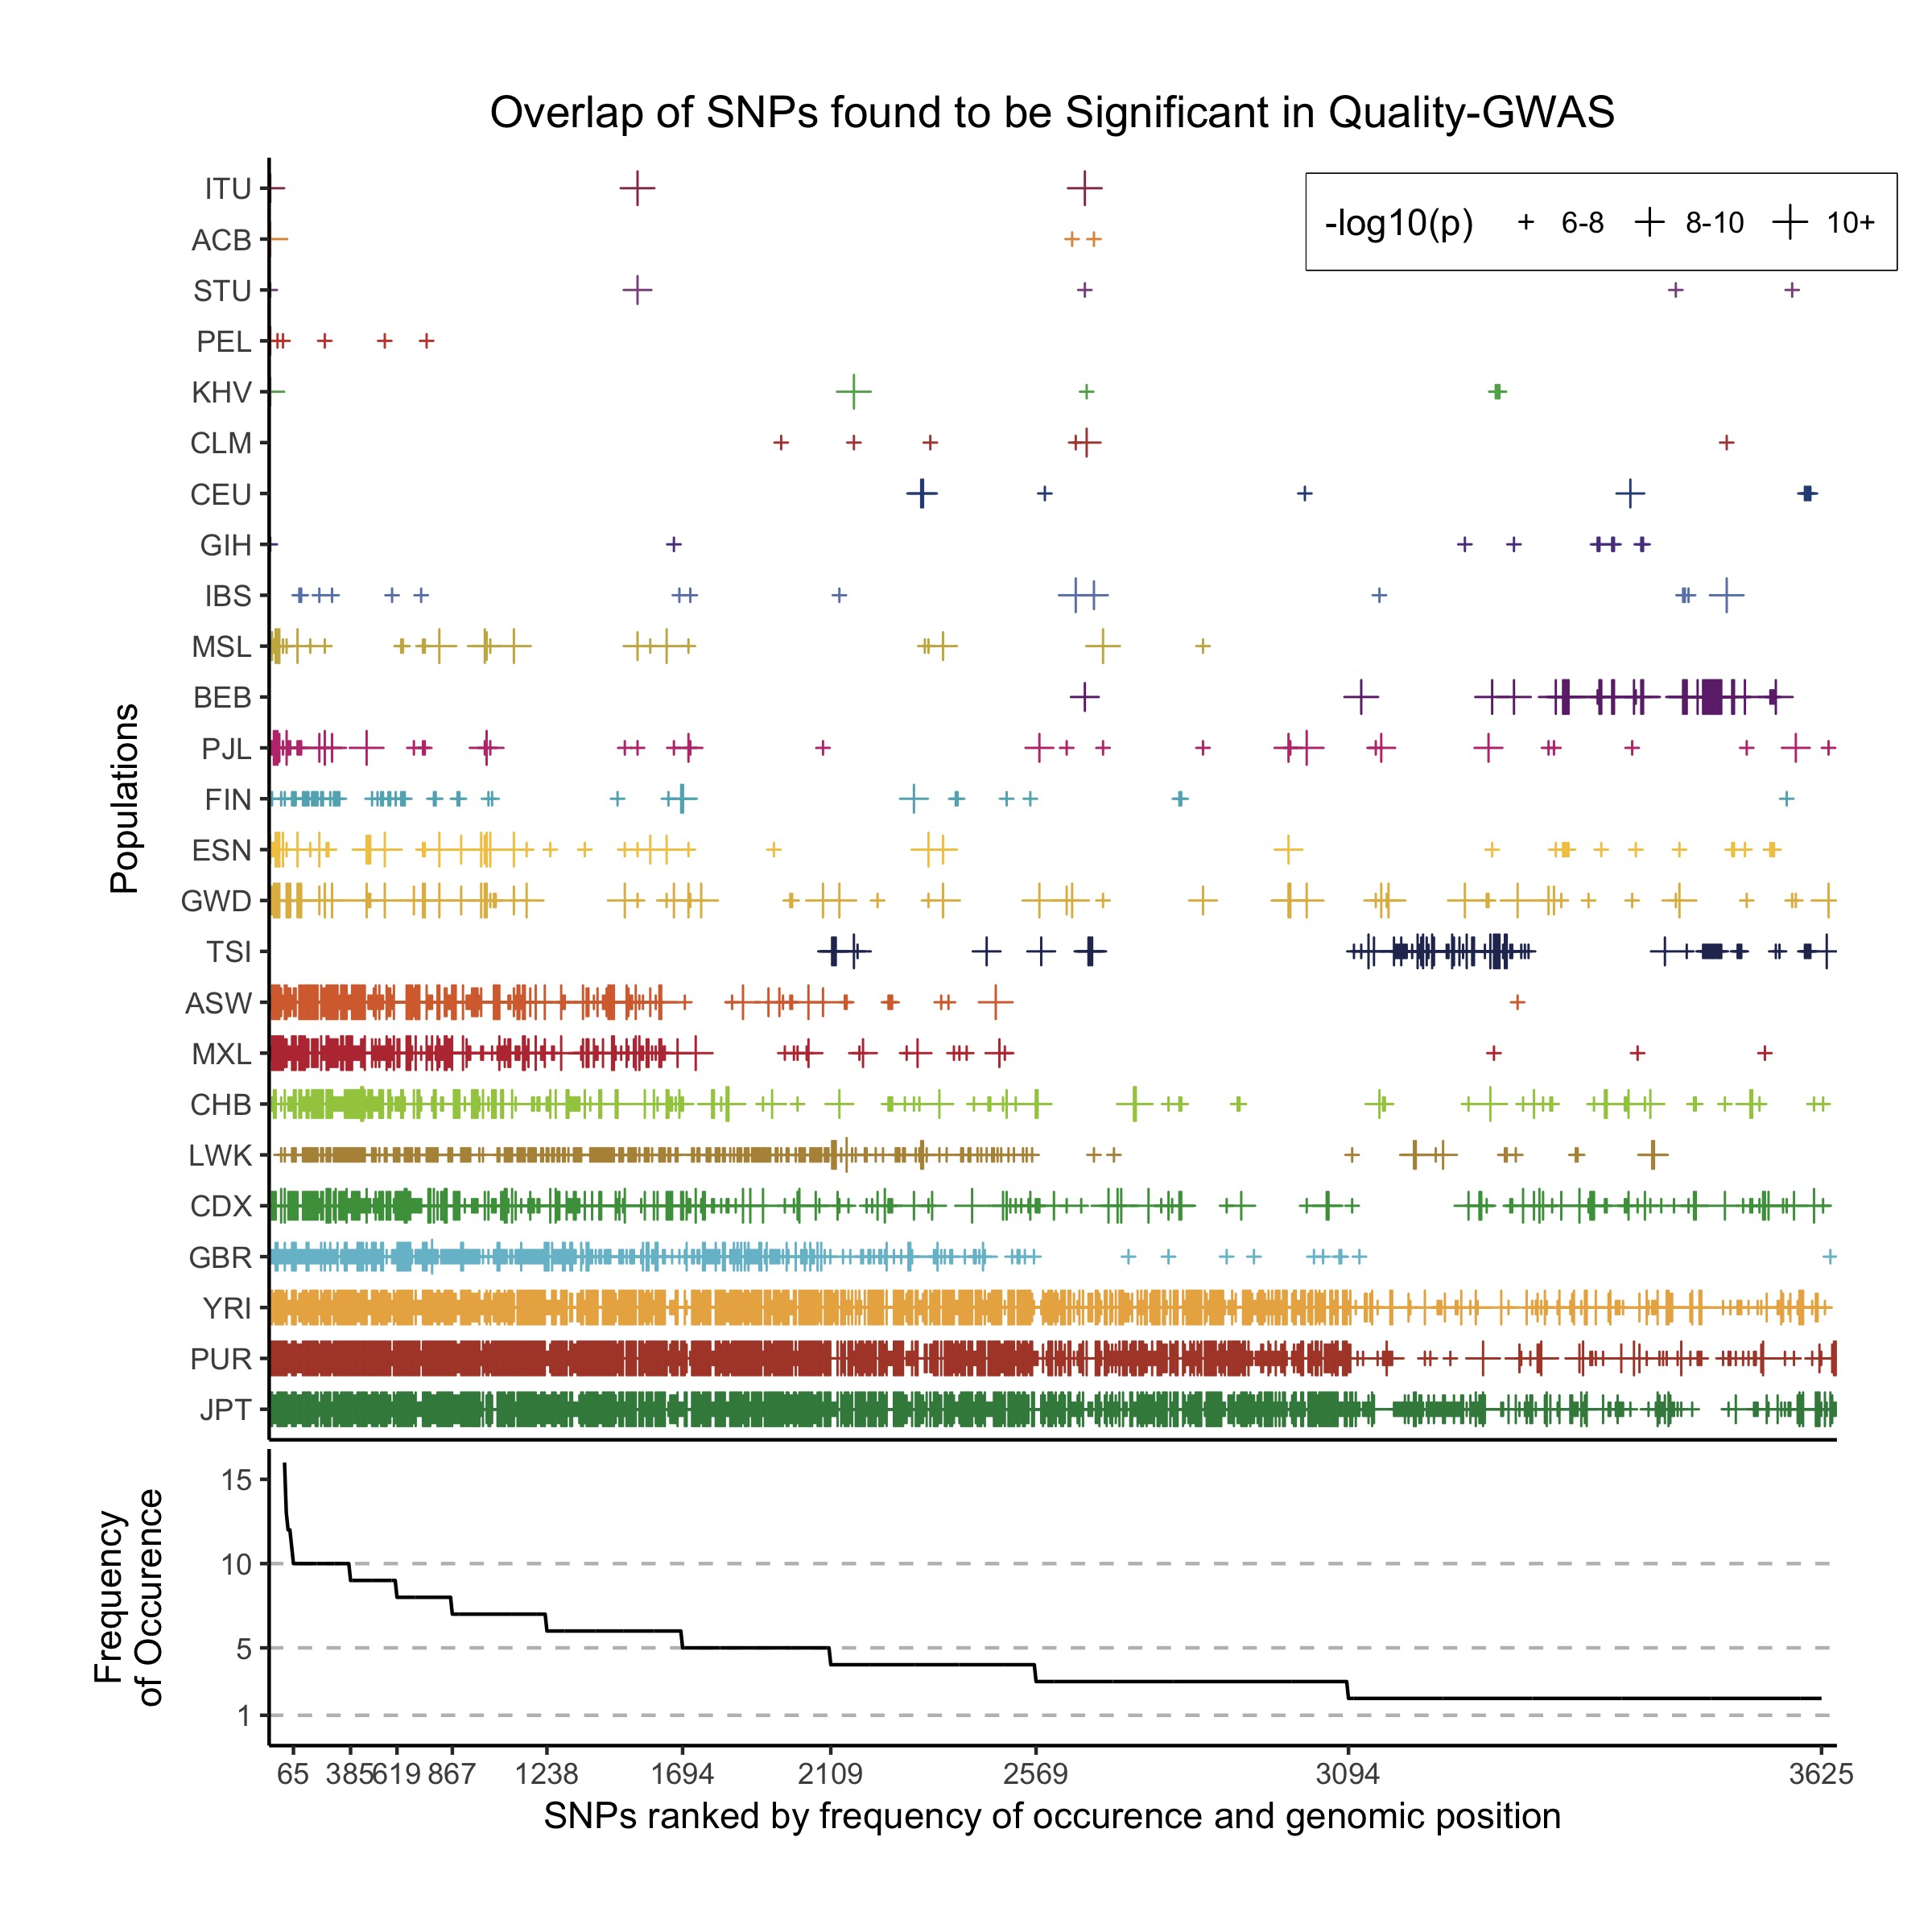
\includegraphics[width=\hsize,keepaspectratio]{SNPOverlap6.jpg}

\caption{Overlap of SNPs identified independently to be associated with quality. 
The populations that have the most low-quality individuals also have the most low-quality variants. 
The same variants identified as being low quality independently in each population are found in other populations. }
  \label{Figure3}
\end{figure*}

	\subsection{Imputation}
~30\% of the SNPs we identified as being associated with low quality were found to be imputed using the Michigan Imputation Server. These should be removed from reference database.

	\subsection{Found to be included in other GWA studies}
Once we identified SNPs that were clearly associated with low quality, we searched the literature for any GWA studies that might have called these erroneous variants as being significantly correlated with some biological trait. 
Using the NHGRI-EBI Catalog of published genome-wide association studies we queried the rsIDs of the SNPs we identified as being low quality and found 6 recent publications that had found at least one of the variants to have reached genome wide significance in their study. 

Five of these studies used the 1kGP as the reference database for imputation and one used the 1kGP cell cultures and sequence data. 
They used strict quality thresholds, including population genetic statistical tests such as the Hardy-Weinberg equilibrium test, deviations in expected allele frequency and sequencing data quality thresholds. 
They also removed rare alleles and alleles with high degrees of missingness. 
Despite using the state of the art quality controls, these erroneous variants managed not only to be imputed onto real genotype data, but they also reached genome wide significance for biological traits. 

			\section{Discussion}
\subsection{Why do we care?}
These SNPs matter because they reached genome wide significance for medically relevant traits. 
Including these variants in the GWAS catalogue could lead to false diagnosis at worst, or spurious correlations at least. 
Polygenic risk scores take into account all SNPs reaching significance, without much manual curation. 
It's likely that the variants we have identified are being included in these multi-locus risk scores.


Despite these variants reaching genome wide significance, the majority of researchers did not pursue these variants for further analysis.
This is likely because these variants have no peak in LD that is characteristic of a biologically significant variant.

\subsection{Recommendations}
The most conservative approach would be to remove all individuals that don't meet the quality threshold as well as all the variants associated to low quality.
In this case, we used a cut off of an average quality of mapped bases over 30. This threshold has been \todo{previously used by studies}. It is the minimum requirements for \todo{GATK variant calling} for them to have a minimum quality of 30.

\subsection{Imputation}
Imputation of genotype data is a probabilistic method that infers the bases of a given genome based on its similarity to a set of reference genomes.
While on average, two humans differ in about 1/10,000 bases, this number is \todo{lower} in closely related individuals, and \todo{higher} in individuals from different continental origins.
Modern chip sequencing will provide the genotype information for over 1 million bases of the genome.
The unique combination of genotyped bases can be enough to identify haplotype blocks that are identical by descent in individuals form the reference database.


The accuracy of imputation depends on the size of the reference database; this varies significantly from one population to another.
This means that individuals with ancestry that is less well represented in the reference database will have lower accuracy of imputation.
To overcome this bias, reference databases are often combined to increase the sample size and in turn, the accuracy of imputation.

\subsection{GWA studies from other papers}
Since these variants are present in more than one population from the 1000 genomes project, they are more likely to be associated to biological traits as they would appear to be like any other variant that is shared among multiple populations. 
The only way to distinguish some of these more covert false positives is to use statistical tests associating the quality metrics of each position relative to each individual. 

\luke{due to the temporal nature of the batch effects, and because entire populations were sequenced in one centre on one day, the false positives are more likely to cluster with population structure or case/control?}

			\section{Conclusion}
Our method identifies spurious mutations by correlating mutations with data quality metrics. 
We propose including our quality control methods to identify possible false positives in sequencing data. 
We have focused on the 1000 Genomes Project dataset as its quality metrics were freely available, however the issues of quality control are not limited to this one consortium. 
This study only used one dataset and one quality metric, but using this same approach can be used to identify more false positives in many more datasets. 

As more large scale genotyping efforts are being imputed on the same legacy datasets, we must scrutinize the quality of the reference databases to avoid the propagation of false positives. 
These results bring forth many questions regarding the reliability of legacy datasets. 
Moreover, since there are so many broad applications of imputation, it frames the question for reference data turnover. 

Many types of DNA sequencing machines have been available on the market over the past decade.
Different types of sequencing technologies can have different technical limitations in quality control.
This makes combining data an issue especially when multiple sequencing technologies are involved in the data production.
Many of the legacy datasets produced using dated sequencing technologies have been known to contain a higher rate of false positives than their more recent counterparts.
The errors in one dataset do not disappear when they are combined with another higher quality one.
The technical biases caused by legacy sequencing technology is becoming increasingly relevant as newer technologies produce data with lower error rates, and more stringent quality controls.




\section{Methods}
\subsection{Metadata}
The metadata used in this analysis was compiled from each of the index files from the 1000 Genomes file system. 
Average quality of mapped bases per sample was obtained from the BAS files associated with each alignment file. 
Each BAS file has metadata regarding each sequencing event for each sample. 
If a sample was sequenced more than once, we took the average of the each quality score from each sequencing instance. 
The submission dates and sequencing centres for each sample in the analysis was available in the sequence index files.  
This file also has multiple entries per sample, however, we were unable to match the individual sequencing runs between the bas files and the index file, which lead us to take the average of the quality scores and only kept the earliest sequencing date per sample. 
The dates of the sequencing are only used to plot Figure. \todo{Average Quality of mapped bases: How was it calculated?}

\subsection{Data Availability}

Index of BAS files \href{http://ftp.1000genomes.ebi.ac.uk/vol1/ftp/data_collections/1000_genomes_project/1000genomes.low_coverage.GRCh38DH.alignment.index}{available here}.

Phase3 analysis sequence index file  \href{http://ftp.1000genomes.ebi.ac.uk/vol1/ftp/phase3/20130502.phase3.analysis.sequence.index}{available here} 

\todo{link to my compiled metadata file here}

\subsection{Quality Controls}
We reproduced the quality control pipelines used by Harris et. al as they applied the current state of the art quality thresholds to remove questionable sequences especially for the high standards for detecting population level differences. 
Several mask files were applied to remove regions of the genome that might be lower quality, or might have very different mutation rates or basepair complexity compared to the rest of the genome. 
The  1000 Genomes \href{http://ftp.1000genomes.ebi.ac.uk/vol1/ftp/release/20130502/supporting/accessible_genome_masks/20141020.strict_mask.whole_genome.bed}{strict mask} was used to remove low quality regions of the genome , highly conserved regions were removed using the \href{http://hgdownload.cse.ucsc.edu/goldenPath/hg19/database/phastConsElements100way.txt.gz}{phastCons100way} mask file and highly repetitive regions were also removed using the \href{http://hgdownload.cse.ucsc.edu/goldenpath/hg19/database/nestedRepeats.txt.gz}{NestedRepeats} mask file from RepeatMasker. 
Furthermore, only diallelic autosomal SNPs were considered, with missingness below 0.01, MAF less than 0.1, and MAF greater than 0.9.

\subsection{Genome Wide Association}

Using PLINK v1.90b4.4 we ran a linear genome wide association study independently for each population of the 1000 Genomes Project. We used the average quality of mapped bases per individual as the phenotype for the analysis. We also controlled for population structure by including the first 4 principle components of a PCA of each population using genotype data. \todo{NOT DONE YET}

\subsection{Mutation Spectrum}
We calculated the mutation spectrum for each list of significant SNPs for each population.  

We also compared the mutation spectrum ratio between populations using a modified version of the methods used in Harris et al. 2017. 

\subsection{Imputation}
Using the Michigan Imputation Server, we imputed the genotype data from 1000 Genomes Project


\section{Code Availability}
\todo{here is where I will put my git hub}

\section{Acknowledgments}
We would like to thank Kelly Harris for sharing her mutation spectrum pipelines.
  
\end{document}
			























